In this section, we will focus on the analysis of different databases based on the  evaluation of XMark queries. BaseX, MongoDB, Couchbase and RethinkDB are completely different database system  with their own data model and different query languages.  Due to their complete different nature, a query of a database would perform better than others if data was normalized according to their specified data model. For example, BaseX would probably perform better if the data is normalized. Therefore, our goal is not to compare queries between these databases but evaluate the results individually.  All databases have been tested with 6 different size XMark dataset as mentioned in ~\ref{benchmark-database-size}. Firstly, the results  of the four systems will be analyzed individually. Further the performances of all the databases of 111MB dataset examined together.

\subsection{MongoDB}
Figure~\ref{fig:xmark-result-mongodb-all} presents the time measurements of XMark queries in MongoDB. MongoDB automatically uses all the free memory of a machine for its cache. The result of the queries will be explained below:
\begin{itemize}
\item The simplest query Q1 was the most efficient query. It was executed in less than 4ms for all database instances, because the MongoDB representation of the query boils down to a simple \textit{\_id} selection.
\item Q2 and Q3 were relatively slow queries due to the number of stages in the aggregation pipeline. Even though two secondary indexes were used, the performance of these queries is not competitive to other systems. 
\item The \textit{count} operation in MongoDB is faster than in other NoSQL databases. Q5 and Q6 are used to count the number of documents in a collection. Q5 contains a comparison operator, and the secondary index in field \textit{price} helped to accelerate the execution. Figure~\ref{fig:xmark-mongodb-index-noindex} illustrates the efficiency of the two queries Q5 and Q13 in which the execution time improved exponentially after the application of the secondary indexes. Q6 is even simpler, as it only contains a \textit{count()} function, and thus hardly consumes any time.

\item Among the join queries, Q8 and Q9 yielded the best result. Once again, the indexes created in these two queries improved the performance. 
But in case of Q10, the complex result generation could not be completed in the given time frame for the two largest database instances. This was probably due to the large result, which does not simply contain database results, but is newly generated by the query. The value join queries in Q11 and Q12 have to deal with many read operations due to the manual looping with the \textit{forEach} expression.

\item The secondary index in Q13 helped to keep execution time low. As mentioned earlier, Fig.~\ref{fig:xmark-result-mongodb-13} shows the consumed time with and without index. Q14 is used to search for sub-strings. Execution time scales linearly.

\item Compared to the XQuery representation, queries Q15 and Q16 are relatively complex in all NoSQL databases including MongoDB, because the child axes of the original query need to rewritten to various aggregation stages. The results produced by these queries were not exactly the same as for XQuery but the performance was in the same order of magnitude. Performance of Q17 was similar to other systems.

\item Q18 ...... \ref{mongodb-q-18}

\item In Q19, a new field \textit{item} is generated. Because of that, performance decreases, because  MongoDB has to use an aggregation pipeline for the new field. The Query would be much faster if the result is returned without a new field by using \textit{find()} function.

\item Finally, cardinalities are grouped and returned in Q20. The mapreduce is implemented for this query. As mentioned in Section~\ref{mongo-query-model}, advanced queries can be achieved in two ways. Q20 is tested in both aggregation pipeline and mapreduce. In pipeline, the query is complex and has to perform in many stages. Mapreduce is flexible, easy to implement and scalable. MongoDB breaks the query in multiple parts handle the processing power accross all the nodes. But in a standalone mode, query is relatively slow. Figure ~\ref{fig:xmark-result-mongodb-pipeline-mapreduce} shows the result of Q20 in both mapreduce and pipeline. The Mapreduce is single-threaded therefore, it is relatively slower to aggregation pipeline.
\end{itemize}
\begin{figure}
	\centering
	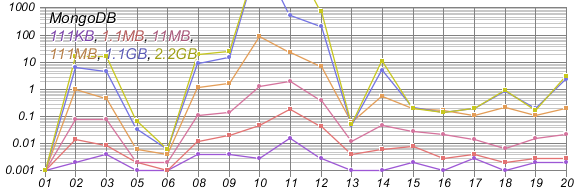
\includegraphics[width=0.95\textwidth]{img/result/mongodb/mongodb-all}
	\caption{XMark queries in MongoDB}
	\label{fig:xmark-result-mongodb-all}
	
\end{figure}	
\begin{figure}
	\centering
	\subfloat[Q5]{
		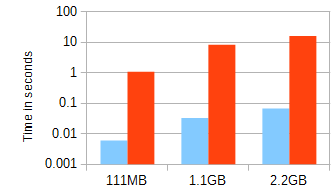
\includegraphics[width=0.49\textwidth]{img/result/mongodb/mongodb-q5-index-noindex}
		\label{fig:xmark-result-mongodb-5}
	}
	\centering
	\subfloat[Q13]{
		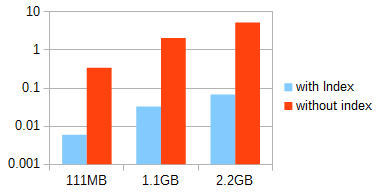
\includegraphics[width=0.49\textwidth]{img/result/mongodb/mongodb-q13-index-noindex}
		\label{fig:xmark-result-mongodb-13}
	}
	\caption{MongoDB queries with and without secondary index in different database instances}
	\label{fig:xmark-mongodb-index-noindex}
\end{figure}

\begin{figure}
	\centering
	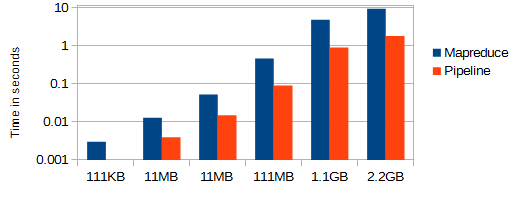
\includegraphics[width=0.95\textwidth]{img/result/mongodb/mongodb-mapreduce-pipeline}
	\caption{Aggregation pipeline and Mapreduce result of Q20 in MongoDB}
	\label{fig:xmark-result-mongodb-pipeline-mapreduce}
	
\end{figure}

\subsection{Basex}
The results of all six different databases in BaseX is shown in Figure~\ref{fig:xmark-result-basex-all}. All the queries were tested with text, attribute and full text indexes. The query Q1 utilizes the attributes index and return a single result. This query was completed in less than 5ms in all databases. The query Q2 and Q3  with positional predicates took longer time if the size of database is increased. The queries Q5 and Q6 uses count operation and both were relatively faster. As seen in previous section, these queries performed better in MongoDB than in BaseX. For databases larger than 11MB, among the join-queries,  Q11 and Q12 could not be completed in specified time frame. For reference join Q8 and Q9, the attribute index is utilized. The time taken by these two queries is  similar to that of MongoDB.  The full text search query Q14 was slightly affected by the size of database. The queries Q15-Q17 implements the location paths, with similar performances and query Q18  implements user defined function for calculation. Q19 consumes most of resources for sorting the data. This query is faster in MongoDB compared to BaseX. Finally, the aggregation query Q20 produces constant result in all database instances. 
\begin{figure}
	\centering
	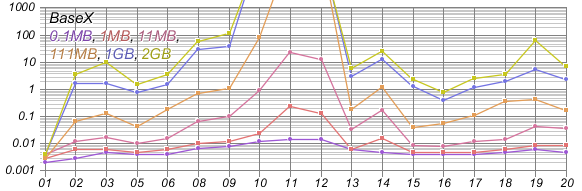
\includegraphics[width=0.95\textwidth]{img/result/basex/basex-all}
	\caption{XMark queries in BaseX}
	\label{fig:xmark-result-basex-all}
\end{figure}

\subsection{RethinkDB}
All the time evaluation of XMark queries in RethinkDB is given in Fig.~\ref{fig:xmark-result-rethinkdb-all}. 
\begin{itemize}
\item Query Q1 consume more time compared to MongoDB and BaseX in average.
 \item  
  RethinkDB is able to handle arrays better way than other NoSQL databases. Chains of queries can be used as a pipeline but unlike MongoDB's pipeline that produces result in multiple stages, RethinkDB runs a query on a server at once, hence it has been seen that queries Q2 and Q3 produces better result compare to MongoDB. 
 \item
 Queries Q5 and Q6 were comparatively slow in  RethinkDB. Firstly, MongoDB uses secondary index on Q5, but RethinkDB cannot use an secondary index in \textit{filter()} function. Secondly, the \textit{count()} operation in RethinkDB is always slow due to stream properties. It executes everything in server, most of the stream operations including \textit{filter} runs lazily. The \textit{run} function returns the results as soon as the first block of data is available, It does not load whole table data  at once. It will only load the data as clients iterate over the cursor. Hence, the memory changes with the usage. In case of \textit{count()}, the query has to wait until all the data is loaded. 
 \item As we have mentioned the support of join query in ~\ref{xmark-rethinkdb}, RethinkDB was not able to take advantages of native joins except query Q11 and Q12. The join operation in Q8, Q9 and Q10 were similar in case of time measurement with rest of system. Q10 is slower due to large output and many new fields. 
 \item In query Q13, index is utilized on \textit{regions} field of the table that produces comparable result to MongoDB but better than BaseX. Queries Q14-Q19 have returned similar result except Q15. Due to many arrays and object operations, Q15 was a bit slower. 
\item The query Q20 was once again slow in RethinkDB due to cardinalities at the end of the query. All the grouping and categorizing operations were a lot faster than the \textit{count()} at the end. 
\end{itemize}

\begin{figure}
	\centering
	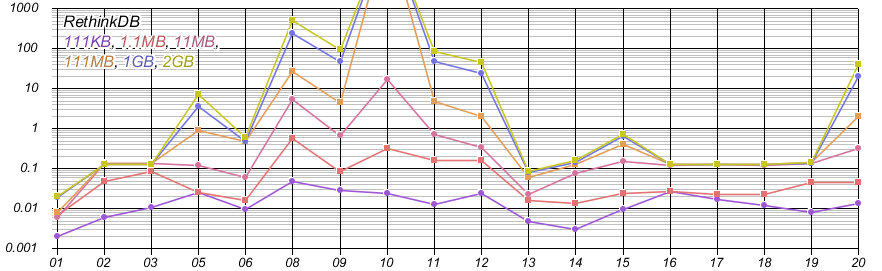
\includegraphics[width=0.95\textwidth]{img/result/rethinkdb/rethinkdb-all}
	\caption{XMark queries in RethinkDB}
	\label{fig:xmark-result-rethinkdb-all}
\end{figure}

\subsection{Couchbase}
Each Couchbase bucket is assigned RAM quota for caching data, therefore, the performance of a query depends on the amount of RAM allocated at the time of bucket creation. Figure~\ref{fig:xmark-result-cb-all} explains the query performance of individual queries\todo{put all database images}. There was not any extraordinary phenomenon in Couchbase.  Query Q1-Q3  were similar to RethinkDB but Q5 and Q6 had produced comparatively better result due to its pre-defined reduce function \textit{\_count} in mapreduce. All the join queries were executed successfully in given time frame. Queries Q15-Q16 have performed slightly  better than that of other databases due to the JavaScript in map function. Another best result in Couchbase is aggregation query Q20, which is able to use pre-defined \textit{\_sum} in reduce part of Mapreduce. 

\begin{figure}
	\centering
	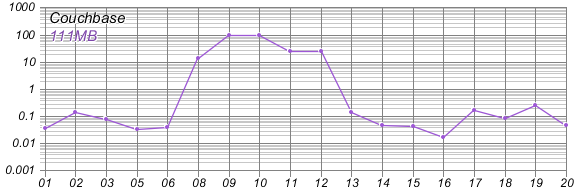
\includegraphics[width=0.95\textwidth]{img/result/cb/cb-all}
	\caption{XMark queries in Couchbase}
	\label{fig:xmark-result-cb-all}
\end{figure}

\subsection{Summary}
Even though our aim is not to compare query performance in different systems directly, it would be interesting to see how these queries look like together. Figure~\ref{fig:xmark-result-1-all-new} illustrates all the queries for different database systems together for 111MB XMark data instance. MongoDB and BaseX had produced the best result in Q1. In Q2 and Q3, all database except MongoDB  had an identical result but in Q5 and Q6 MongoDB was the clear leader followed by Couchbae and BaseX, whereas RethinkDB was lagging behind other databases. In the join queries, the results produced by different databases were mixed in nature. MongoDB and BaseX were relatively better in Q8 and Q9 followed by Couchbase and RethinkDB. In Query Q10, the RethinkDB has failed to return result in a given time frame, but all other databases has similar results. The value join queries Q11 and Q12 were the best queries for RethinkDB followed by MongoDB and Couchbase, but BaseX could not complete the result. Even the Q13 has similar results for all systems, RethinkDB had generated the best performance followed by MongoDB due to their efficient indexes. The FT search query Q14 is substring search for NoSQL databases, so that the query is a bit faster on them. The complex XPath queries Q15 and Q16 of Basex has better result with Couchbase than RethinkDB and MongoDB.
Q17-Q19 results are identical but in Q20 the Couchbase was the leader followed by Basex, MongoDB and RethinkDB. 
\par
It has been seen that the NoSQL queries that were able to use secondary indexes performed better than BaseX with some exception. Even though some NoSQL databases do not support join queries, the results they produced were competitive in nature. The reason was favourable data model defined for those databases compare to BaseX. BaseX would probably perform better if the queries or data were normalized.
% NoSQL database has efficient read operation 
\begin{table}[H]
\tiny
\begin{tabular}{|c|c|c|c|c|c|c|c|c|c|c| c|c|c|c|c|c|c|c|c|c|c|  } 
   db &  1 & 2 & 3 & 5 & 6  & 8 & 9 & 10  & 11 & 12 & 13 & 14 & 15 & 16 & 17 & 18 & 19 & 20 \\
 \hline
M\hbox{\pdfliteral{1 1 0 rg}\vrule height2mm width2mm depth0mm\pdfliteral{0 g}} & .00 & .75 & .78 & .01 & .00 & 1.17 & 1.65 & 87.25 & 23.13 & 7.21 & .05 & .55 & .20 & .17 & .11 & .22 & .11 & .21 \\
B\hbox{\pdfliteral{0 0 1 rg}\vrule height2mm width2mm depth0mm\pdfliteral{0 g}} & .04 & .19 & .17 & .10 & .19 & 2.31 & 2.43 & 89.36 & udf & udf & .36 & 1.23 & .08 & .08 & .15 & .36 & .52 & .19 \\
C\hbox{\pdfliteral{1 0 0 rg}\vrule height2mm width2mm depth0mm\pdfliteral{0 g}} & .04 & .14 & .08 & .03 & .04 & 13.2 & 98.1 & 94.1 & 24.1 & 26.1 & .13 & .05 & .04 & .02 & .17 & .09 & .27 & .05 \\
R\hbox{\pdfliteral{0 1 0 rg}\vrule height2mm width2mm depth0mm\pdfliteral{0 g}} & .01 & .14 & .14 & .94 & .68 & 26.76 & 4.53 & .00 & 4.80 & 2.10 & .02 & .18 & udf & .13 & .13 & .13 & .14 & 2.04 \\
\end{tabular}
\end{table}
\begin{figure}[H]
	\centering
	\subfloat[XMark queries of 111MB data in all DBMS]{
		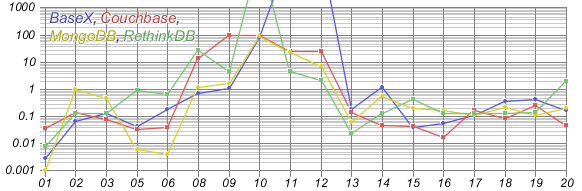
\includegraphics[width=0.85\textwidth]{img/result/1/1-all-new}		\label{fig:xmark-result-1-all-new}
	}
	\caption{XMark queries of 111MB data in all DBMS}
	\label{fig-xmark-result-1-all-queries}
\end{figure}